\fancyhead[LH]{计算机控制系统课程报告}
\fancyhead[RH]{1\quad 绪论}
\section{绪论}

\subsection{研究背景与意义}

\subsection{杭州“六小龙”概况}

图片引用测试\ref{fig:myfig2}:

\begin{figure}[H] % 这里 H 表示 强制放置在当前位置,更改为htbp表示根据需要放置
    \centering
    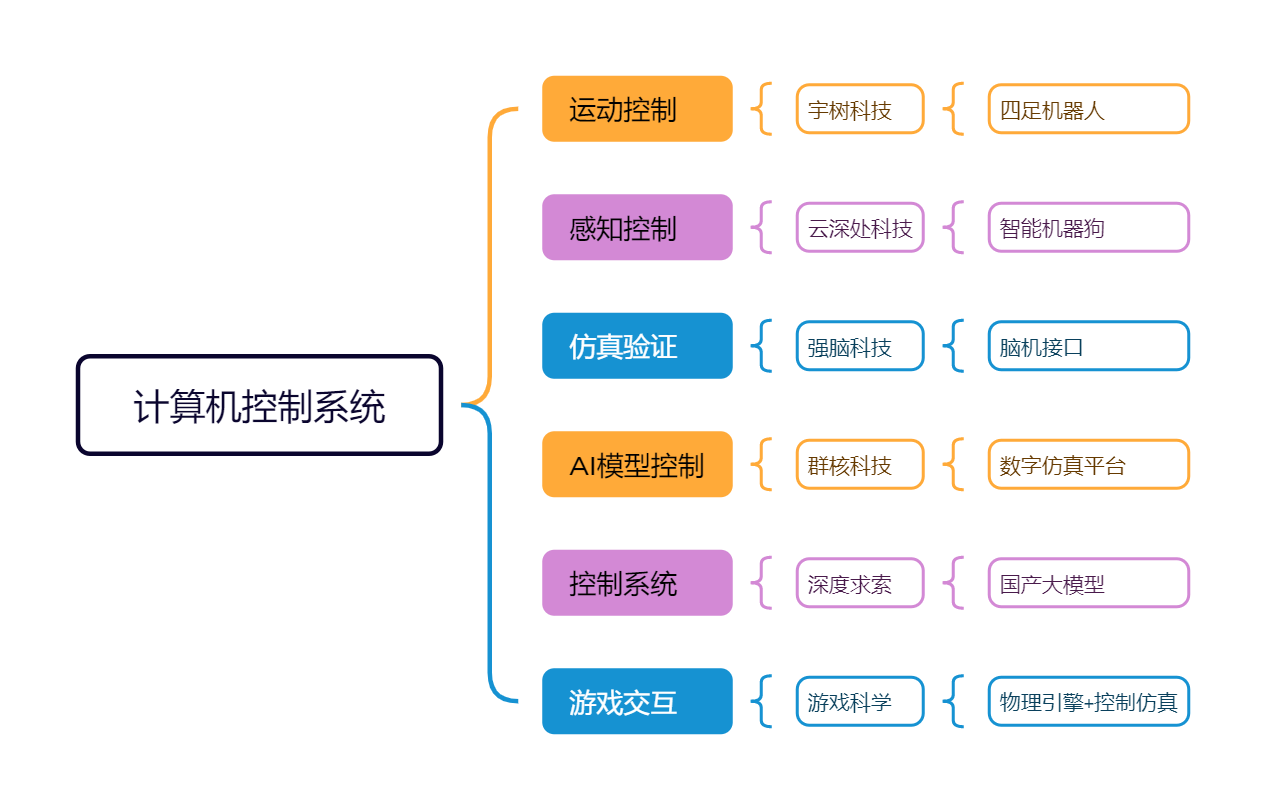
\includegraphics[width=0.8\textwidth]{fig/fig2.png} % 可调整宽度
    \caption{“六小龙”核心技术与计算机控制系统的关系}
    \label{fig:myfig2}
\end{figure}

文献引用示例\cite{ccs}

公式示例\ref{eq:pid-incremental}:
\begin{equation}
    \left\{
    \begin{aligned}
        u(k) &= q_0 e(k) + B(k-1) \\
        B(k) &= u(k) + q_1 e(k-1) + q_2 e(k-2) \\
        q_0 &= K_p \left(1 + \frac{T_s}{T_i} + \frac{T_d}{T_s} \right) \\
        q_1 &= -K_p \left(1 + 2 \cdot \frac{T_d}{T_s} \right) \\
        q_2 &= K_p \cdot \frac{T_d}{T_s}
    \end{aligned}
    \right.
    \label{eq:pid-incremental}
    \end{equation} 

表格示例:
\begin{table}[H]
    \centering
    \caption{高频感应加热的基本参数}
    \begin{tabular}{|c| c|c|c|}
    \hline
    感应频率 &感应发生器功率 & 工件移动速度  &感应圈与零件间隙\\
    (KHz)&($\% \times$80Kw) &(mm/min)  &(mm)\\
    \hline
    250 &88 &5900 &1.65\\
    \hline
    250 &88 &5900 &1.65\\
    \hline
    250 &88 &5900 &1.65\\
    \hline
    250 &88 &5900 &1.65\\
    \hline
    \end{tabular}
\end{table}


\begin{table}
    \centering
    \captionsetup{singlelinecheck=off}
    \caption*{续表} %取消编号
    \begin{tabular}{|c| c|c|c|}
    \hline
    感应频率 &感应发生器功率 & 工件移动速度  &感应圈与零件间隙\\
    (KHz)&($\% \times$80Kw) &(mm/min)  &(mm)\\
    \hline
    250 &88 &5900 &1.65\\
    \hline
    250 &88 &5900 &1.65\\
    \hline
    \end{tabular}
\end{table}
%表格太大需要转页时,需要在续表上方注明“续表”,表头也应重复排出。 % 这里的 tab/tab1.tex 是表格文件的路径

\subsection{报告结构与研究方法}

\newpage